% Created by tikzDevice version 0.12 on 2019-06-13 12:46:35
% !TEX encoding = UTF-8 Unicode
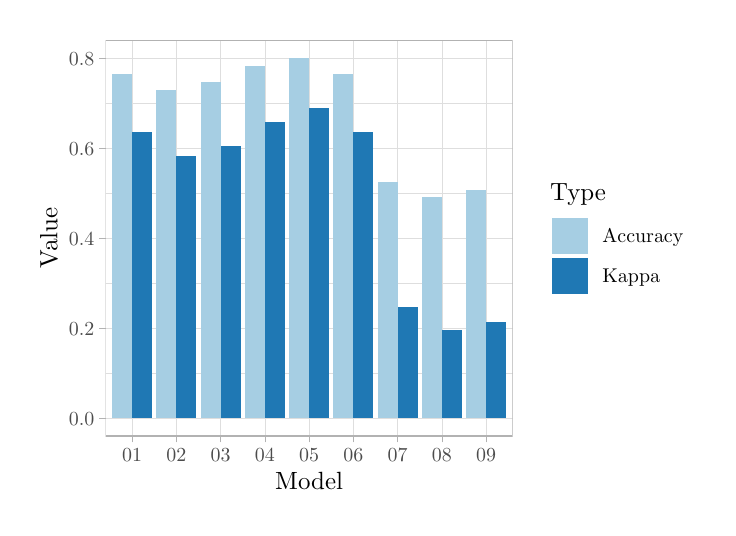
\begin{tikzpicture}[x=1pt,y=1pt]
\definecolor{fillColor}{RGB}{255,255,255}
\path[use as bounding box,fill=fillColor,fill opacity=0.00] (0,0) rectangle (245.72,173.45);
\begin{scope}
\path[clip] (  0.00,  0.00) rectangle (245.72,173.45);
\definecolor{drawColor}{RGB}{255,255,255}
\definecolor{fillColor}{RGB}{255,255,255}

\path[draw=drawColor,line width= 0.5pt,line join=round,line cap=round,fill=fillColor] (  0.00,  0.00) rectangle (245.72,173.45);
\end{scope}
\begin{scope}
\path[clip] ( 28.14, 25.85) rectangle (175.25,168.95);
\definecolor{fillColor}{RGB}{255,255,255}

\path[fill=fillColor] ( 28.14, 25.85) rectangle (175.25,168.95);
\definecolor{drawColor}{gray}{0.87}

\path[draw=drawColor,line width= 0.1pt,line join=round] ( 28.14, 48.59) --
	(175.25, 48.59);

\path[draw=drawColor,line width= 0.1pt,line join=round] ( 28.14, 81.06) --
	(175.25, 81.06);

\path[draw=drawColor,line width= 0.1pt,line join=round] ( 28.14,113.54) --
	(175.25,113.54);

\path[draw=drawColor,line width= 0.1pt,line join=round] ( 28.14,146.02) --
	(175.25,146.02);

\path[draw=drawColor,line width= 0.2pt,line join=round] ( 28.14, 32.35) --
	(175.25, 32.35);

\path[draw=drawColor,line width= 0.2pt,line join=round] ( 28.14, 64.83) --
	(175.25, 64.83);

\path[draw=drawColor,line width= 0.2pt,line join=round] ( 28.14, 97.30) --
	(175.25, 97.30);

\path[draw=drawColor,line width= 0.2pt,line join=round] ( 28.14,129.78) --
	(175.25,129.78);

\path[draw=drawColor,line width= 0.2pt,line join=round] ( 28.14,162.25) --
	(175.25,162.25);

\path[draw=drawColor,line width= 0.2pt,line join=round] ( 37.73, 25.85) --
	( 37.73,168.95);

\path[draw=drawColor,line width= 0.2pt,line join=round] ( 53.72, 25.85) --
	( 53.72,168.95);

\path[draw=drawColor,line width= 0.2pt,line join=round] ( 69.71, 25.85) --
	( 69.71,168.95);

\path[draw=drawColor,line width= 0.2pt,line join=round] ( 85.71, 25.85) --
	( 85.71,168.95);

\path[draw=drawColor,line width= 0.2pt,line join=round] (101.70, 25.85) --
	(101.70,168.95);

\path[draw=drawColor,line width= 0.2pt,line join=round] (117.69, 25.85) --
	(117.69,168.95);

\path[draw=drawColor,line width= 0.2pt,line join=round] (133.68, 25.85) --
	(133.68,168.95);

\path[draw=drawColor,line width= 0.2pt,line join=round] (149.67, 25.85) --
	(149.67,168.95);

\path[draw=drawColor,line width= 0.2pt,line join=round] (165.66, 25.85) --
	(165.66,168.95);
\definecolor{fillColor}{RGB}{31,120,180}

\path[fill=fillColor] ( 37.73, 32.35) rectangle ( 44.93,135.63);
\definecolor{fillColor}{RGB}{166,206,227}

\path[fill=fillColor] ( 30.54, 32.35) rectangle ( 37.73,156.75);
\definecolor{fillColor}{RGB}{31,120,180}

\path[fill=fillColor] ( 53.72, 32.35) rectangle ( 60.92,127.14);
\definecolor{fillColor}{RGB}{166,206,227}

\path[fill=fillColor] ( 46.53, 32.35) rectangle ( 53.72,151.05);
\definecolor{fillColor}{RGB}{31,120,180}

\path[fill=fillColor] ( 69.71, 32.35) rectangle ( 76.91,130.83);
\definecolor{fillColor}{RGB}{166,206,227}

\path[fill=fillColor] ( 62.52, 32.35) rectangle ( 69.71,153.90);
\definecolor{fillColor}{RGB}{31,120,180}

\path[fill=fillColor] ( 85.71, 32.35) rectangle ( 92.90,139.48);
\definecolor{fillColor}{RGB}{166,206,227}

\path[fill=fillColor] ( 78.51, 32.35) rectangle ( 85.71,159.59);
\definecolor{fillColor}{RGB}{31,120,180}

\path[fill=fillColor] (101.70, 32.35) rectangle (108.89,144.25);
\definecolor{fillColor}{RGB}{166,206,227}

\path[fill=fillColor] ( 94.50, 32.35) rectangle (101.70,162.44);
\definecolor{fillColor}{RGB}{31,120,180}

\path[fill=fillColor] (117.69, 32.35) rectangle (124.88,135.67);
\definecolor{fillColor}{RGB}{166,206,227}

\path[fill=fillColor] (110.49, 32.35) rectangle (117.69,156.75);
\definecolor{fillColor}{RGB}{31,120,180}

\path[fill=fillColor] (133.68, 32.35) rectangle (140.87, 72.53);
\definecolor{fillColor}{RGB}{166,206,227}

\path[fill=fillColor] (126.48, 32.35) rectangle (133.68,117.81);
\definecolor{fillColor}{RGB}{31,120,180}

\path[fill=fillColor] (149.67, 32.35) rectangle (156.86, 64.22);
\definecolor{fillColor}{RGB}{166,206,227}

\path[fill=fillColor] (142.47, 32.35) rectangle (149.67,112.12);
\definecolor{fillColor}{RGB}{31,120,180}

\path[fill=fillColor] (165.66, 32.35) rectangle (172.85, 67.25);
\definecolor{fillColor}{RGB}{166,206,227}

\path[fill=fillColor] (158.46, 32.35) rectangle (165.66,114.96);
\definecolor{drawColor}{gray}{0.70}

\path[draw=drawColor,line width= 0.5pt,line join=round,line cap=round] ( 28.14, 25.85) rectangle (175.25,168.95);
\end{scope}
\begin{scope}
\path[clip] (  0.00,  0.00) rectangle (245.72,173.45);
\definecolor{drawColor}{gray}{0.30}

\node[text=drawColor,anchor=base east,inner sep=0pt, outer sep=0pt, scale=  0.72] at ( 24.09, 29.87) {0.0};

\node[text=drawColor,anchor=base east,inner sep=0pt, outer sep=0pt, scale=  0.72] at ( 24.09, 62.35) {0.2};

\node[text=drawColor,anchor=base east,inner sep=0pt, outer sep=0pt, scale=  0.72] at ( 24.09, 94.82) {0.4};

\node[text=drawColor,anchor=base east,inner sep=0pt, outer sep=0pt, scale=  0.72] at ( 24.09,127.30) {0.6};

\node[text=drawColor,anchor=base east,inner sep=0pt, outer sep=0pt, scale=  0.72] at ( 24.09,159.77) {0.8};
\end{scope}
\begin{scope}
\path[clip] (  0.00,  0.00) rectangle (245.72,173.45);
\definecolor{drawColor}{gray}{0.70}

\path[draw=drawColor,line width= 0.2pt,line join=round] ( 25.89, 32.35) --
	( 28.14, 32.35);

\path[draw=drawColor,line width= 0.2pt,line join=round] ( 25.89, 64.83) --
	( 28.14, 64.83);

\path[draw=drawColor,line width= 0.2pt,line join=round] ( 25.89, 97.30) --
	( 28.14, 97.30);

\path[draw=drawColor,line width= 0.2pt,line join=round] ( 25.89,129.78) --
	( 28.14,129.78);

\path[draw=drawColor,line width= 0.2pt,line join=round] ( 25.89,162.25) --
	( 28.14,162.25);
\end{scope}
\begin{scope}
\path[clip] (  0.00,  0.00) rectangle (245.72,173.45);
\definecolor{drawColor}{gray}{0.70}

\path[draw=drawColor,line width= 0.2pt,line join=round] ( 37.73, 23.60) --
	( 37.73, 25.85);

\path[draw=drawColor,line width= 0.2pt,line join=round] ( 53.72, 23.60) --
	( 53.72, 25.85);

\path[draw=drawColor,line width= 0.2pt,line join=round] ( 69.71, 23.60) --
	( 69.71, 25.85);

\path[draw=drawColor,line width= 0.2pt,line join=round] ( 85.71, 23.60) --
	( 85.71, 25.85);

\path[draw=drawColor,line width= 0.2pt,line join=round] (101.70, 23.60) --
	(101.70, 25.85);

\path[draw=drawColor,line width= 0.2pt,line join=round] (117.69, 23.60) --
	(117.69, 25.85);

\path[draw=drawColor,line width= 0.2pt,line join=round] (133.68, 23.60) --
	(133.68, 25.85);

\path[draw=drawColor,line width= 0.2pt,line join=round] (149.67, 23.60) --
	(149.67, 25.85);

\path[draw=drawColor,line width= 0.2pt,line join=round] (165.66, 23.60) --
	(165.66, 25.85);
\end{scope}
\begin{scope}
\path[clip] (  0.00,  0.00) rectangle (245.72,173.45);
\definecolor{drawColor}{gray}{0.30}

\node[text=drawColor,anchor=base,inner sep=0pt, outer sep=0pt, scale=  0.72] at ( 37.73, 16.84) {01};

\node[text=drawColor,anchor=base,inner sep=0pt, outer sep=0pt, scale=  0.72] at ( 53.72, 16.84) {02};

\node[text=drawColor,anchor=base,inner sep=0pt, outer sep=0pt, scale=  0.72] at ( 69.71, 16.84) {03};

\node[text=drawColor,anchor=base,inner sep=0pt, outer sep=0pt, scale=  0.72] at ( 85.71, 16.84) {04};

\node[text=drawColor,anchor=base,inner sep=0pt, outer sep=0pt, scale=  0.72] at (101.70, 16.84) {05};

\node[text=drawColor,anchor=base,inner sep=0pt, outer sep=0pt, scale=  0.72] at (117.69, 16.84) {06};

\node[text=drawColor,anchor=base,inner sep=0pt, outer sep=0pt, scale=  0.72] at (133.68, 16.84) {07};

\node[text=drawColor,anchor=base,inner sep=0pt, outer sep=0pt, scale=  0.72] at (149.67, 16.84) {08};

\node[text=drawColor,anchor=base,inner sep=0pt, outer sep=0pt, scale=  0.72] at (165.66, 16.84) {09};
\end{scope}
\begin{scope}
\path[clip] (  0.00,  0.00) rectangle (245.72,173.45);
\definecolor{drawColor}{RGB}{0,0,0}

\node[text=drawColor,anchor=base,inner sep=0pt, outer sep=0pt, scale=  0.90] at (101.70,  6.44) {Model};
\end{scope}
\begin{scope}
\path[clip] (  0.00,  0.00) rectangle (245.72,173.45);
\definecolor{drawColor}{RGB}{0,0,0}

\node[text=drawColor,rotate= 90.00,anchor=base,inner sep=0pt, outer sep=0pt, scale=  0.90] at ( 10.70, 97.40) {Value};
\end{scope}
\begin{scope}
\path[clip] (  0.00,  0.00) rectangle (245.72,173.45);
\definecolor{fillColor}{RGB}{255,255,255}

\path[fill=fillColor] (184.25, 72.12) rectangle (241.22,122.67);
\end{scope}
\begin{scope}
\path[clip] (  0.00,  0.00) rectangle (245.72,173.45);
\definecolor{drawColor}{RGB}{0,0,0}

\node[text=drawColor,anchor=base west,inner sep=0pt, outer sep=0pt, scale=  0.90] at (188.75,111.00) {Type};
\end{scope}
\begin{scope}
\path[clip] (  0.00,  0.00) rectangle (245.72,173.45);
\definecolor{fillColor}{RGB}{255,255,255}

\path[fill=fillColor] (188.75, 91.08) rectangle (203.21,105.53);
\end{scope}
\begin{scope}
\path[clip] (  0.00,  0.00) rectangle (245.72,173.45);
\definecolor{fillColor}{RGB}{166,206,227}

\path[fill=fillColor] (189.46, 91.79) rectangle (202.49,104.82);
\end{scope}
\begin{scope}
\path[clip] (  0.00,  0.00) rectangle (245.72,173.45);
\definecolor{fillColor}{RGB}{255,255,255}

\path[fill=fillColor] (188.75, 76.62) rectangle (203.21, 91.08);
\end{scope}
\begin{scope}
\path[clip] (  0.00,  0.00) rectangle (245.72,173.45);
\definecolor{fillColor}{RGB}{31,120,180}

\path[fill=fillColor] (189.46, 77.33) rectangle (202.49, 90.36);
\end{scope}
\begin{scope}
\path[clip] (  0.00,  0.00) rectangle (245.72,173.45);
\definecolor{drawColor}{RGB}{0,0,0}

\node[text=drawColor,anchor=base west,inner sep=0pt, outer sep=0pt, scale=  0.72] at (207.71, 95.82) {Accuracy};
\end{scope}
\begin{scope}
\path[clip] (  0.00,  0.00) rectangle (245.72,173.45);
\definecolor{drawColor}{RGB}{0,0,0}

\node[text=drawColor,anchor=base west,inner sep=0pt, outer sep=0pt, scale=  0.72] at (207.71, 81.37) {Kappa};
\end{scope}
\end{tikzpicture}
